\documentclass{standalone}
\usepackage{tikz}
\begin{document}
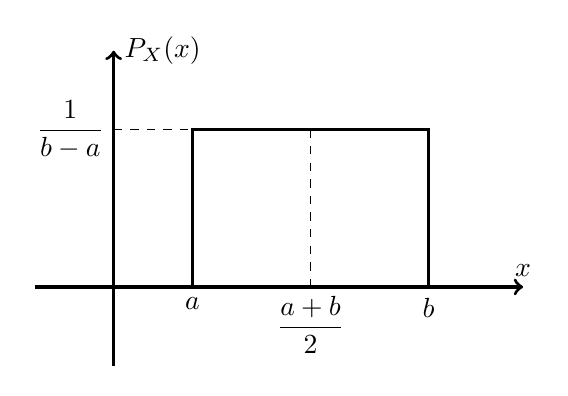
\begin{tikzpicture}[scale=2]
    \draw[->,very thick](-1.5,0)--(1.6,0)node[above]{$x$};
    \draw[->,very thick](-1,-0.5)--(-1,1.5)node[right]{$P_X(x)$};
    \draw[very thick](-0.5,0)node[below]{$a$}--(-0.5,1)--(1,1)--(1,0)node[below]{$b$};
    \draw[dashed](-1,1)node[left]{$\displaystyle\frac{1}{b-a}$}--(-0.5,1);
    \draw[dashed](0.25,1)--(0.25,0)node[below]{$\displaystyle\frac{a+b}{2}$};
\end{tikzpicture}
\end{document}